\documentclass[11pt, floatsintext]{apa6}
\usepackage{amssymb}
\usepackage{graphicx}
\usepackage[outdir=./]{epstopdf}
%\DeclareGraphicsExtensions{.eps}

\usepackage{mathtools}
\usepackage{enumerate}
\usepackage{apacite}
\usepackage{listings}
\usepackage{multirow}
\usepackage{todonotes}
\usepackage{svg}
\usepackage{booktabs}


\newcommand{\den}[2][]{
\(
\left\llbracket\;\text{#2}\;\right\rrbracket^{#1}
\)
}

\synctex=1
\usepackage{soul}

\newcommand{\KL}[2]{\ensuremath{D_{KL}({#1}\, \| \, {#2})}}
\newcommand{\E}[2]{\ensuremath{\mathbb{E}_{#1}\left [#2 \right]}}

\newenvironment{figurehere}
	{\def\@captype{figure}}
	{}

\usepackage{lipsum}
%\pagenumbering{gobble}
%\usepackage{apacite}

\linespread{1}
\usepackage{textcomp}
\usepackage{lingmacros}

\DeclareGraphicsRule{.tif}{png}{.png}{`convert #1 `dirname #1`/`basename #1 .tif`.png}
\graphicspath{{./figures/}}
 
 \definecolor{Green}{RGB}{10,200,100}
  \definecolor{Red}{RGB}{200,100,50}
\newcommand{\ndg}[1]{\textcolor{Green}{[ndg: #1]}}  
\newcommand{\rdh}[1]{\textcolor{Red}{[rdh: #1]}}  


\makeatother

\title{An inferential theory of convention formation}
\shorttitle{Conventions}
\author{Authors}
\affiliation{Universities}

\abstract{Abstract}


\keywords{keywords}

\authornote{This report is based in part on work presented at the 38th Conference of the Cognitive Science Society. Correspondence should be addressed to Robert D. Hawkins, e-mail: rdhawkins@princeton.edu}

\begin{document}
\maketitle

\section{Introduction}

\subsection{Cognitive theories of local alignment}

Interactive alignment theories say that coordination is `priming' with some connectionist voodoo that trickles up levels. 

\subsection{Distributed network theories of global convergence}

Agent-based models use heuristics 

\section{Convention formation as hierarchical inference}

We present our model. It is learning and inference all the way down but gives rise to emergent behavior in groups.

\section{Experiment 1: pragmatic inferences shape conventions}

We run some simulations and fit our model to an artificial language communication game. 

We make the point that our model (by virtue of bayesian inference machinery) explains the way context shapes conventions in ways that other models cannot.

\subsection{Simulations}

We show conditions under which you see convergence. 

\subsection{Experimental design}

\section{Experiment 2: generalization to new partners in a social network}

How do \emph{ad hoc} conventions formed through interaction with a single partner become \emph{global} conventions that can be expected to hold more widely?
In this section, we provide an explicit account of the cognitive mechanisms underlying this transformation.
The key prediction of our model concerns the pattern of generalization across partners.
In Section \ref{} we showed that our model accounts for the \emph{partner-specificity} of ad hoc conventions: observing a single instead of continuing to use an efficient label, they revert back to a longer initial description with a novel partner.
However, we predict that the partner-specific expectations agents form within an interaction to solve a novel communication problem will gradually generalize to community-wide expectations as they interact with more members of their community. 
After talking to enough partners in a tight-knit community, speakers may infer latent structure shared across different partners: certain labels that multiple listener seem to understand. 
If speakers then attempt to adhere to this inferred structure,  more willing to assume novel partners will share the same lexicon.

\subsection{Simulations}

\begin{figure}[t!]
\centering
    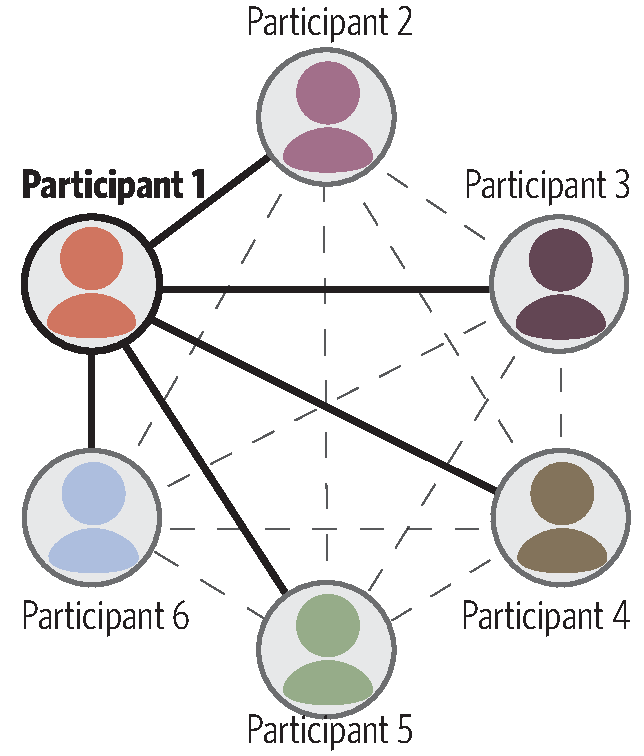
\includegraphics[scale=.32]{task1_network.pdf}
  \caption{Network}% tying individual cognition to population-level patterns}
  \label{fig:task1_network}
\end{figure}

\subsection{Experiment design}
%At a high level, my experiment design will follow the basic setup from \cite{fay_interactive_2010}. 
Using the Dallinger platform, I will recruit 600 participants from Amazon Mechanical Turk to play an interactive, multi-player reference game. 
Participants will be randomly assigned to one of 100 six-member communities embedded as a complete graph, such that everyone is neighbors with everyone else in their community (Fig. \ref{fig:task1_network}). 
Each participant will be paired with a neighbor for a repeated reference game where they must coordinate on conventions for talking about six abstract tangram shapes.
%On each trial of this task, one participant (the `speaker') will be privately shown a highlighted target object and must communicate the identity of this object to their partner (the `listener'), who may reply but must ultimately make a selection from the array. 
The trial sequence for this partner will be constructed so that each of six targets appear six times, spread evenly across the session, for a total of 36 trials.
After completing 36 trials with one partner, they will be introduced to a new partner with a different avatar and asked to play the repeated reference game again with the same six objects.
This process will repeat until they have been partnered with all five neighbors.
Players will be given full feedback about their partner's choice and receive bonus payment for each correct response. 
We will exclude participants reporting a native language different from English. 

\begin{figure}
\centering
    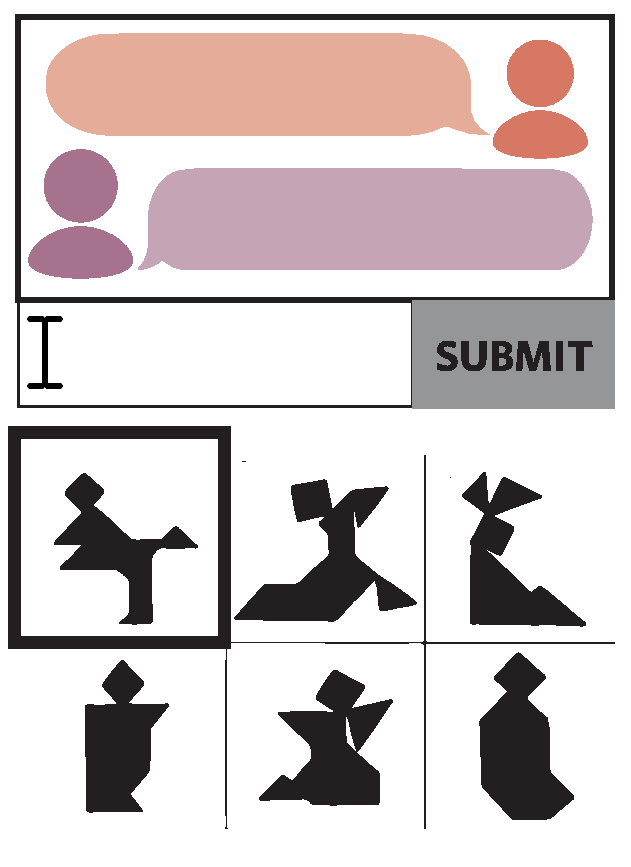
\includegraphics[scale=.27]{task1_display.pdf}
  \caption{Task}% tying individual cognition to population-level patterns}
  \label{fig:task1_display}
\end{figure}

\subsection{Stimuli}
We will use an array of six tangram objects used by \citeA[Fig. \ref{fig:task1_display}]{clark_referring_1986}. There are two reasons to use classic tangram stimuli rather than constructing a novel stimulus set: (1) it allows us to make more direct comparison of our results with the long existing literature using these stimuli  \shortcite<e.g.>{duff_development_2006,hawkins_convention-formation_2017} and (2) they have already been normed to lie in a ``sweet spot'' of ambiguity where speakers do not have strong pre-existing lexical conventions for how to refer to these figures (unlike an image a dog), but they are structured enough to allow success under many creative interpretations (unlike an image of white noise).

\subsection{Confirmatory behavioral predictions}
%A partial pooling account makes three behavioral predictions that allow us to distinguish it from no pooling and complete pooling accounts. 
The most diagnostic analysis to distinguish between the three models concerns the mean number of words used per description, which is a common operationalization of conventionalization in reference games.
In particular, we are interested in how this measure changes within partners and across partner boundaries.
The first panel of Fig. \ref{fig:task1predictions} shows the mean number of words used across six repetitions with one partner in a pilot experiment with $N=100$ isolated pairs.
All three models are consistent with this pattern: messages reduce in length across repetitions with a partner as they coordinate on shorthand. 

However, the three accounts diverge in their predictions at the partner boundary, as visualized in the remaining panels of Fig. \ref{fig:task1predictions}. Pilot data was used to calibrate expected effect sizes. 
While complete pooling predicts that participants will completely transfer conventions from the previous partner  \cite<inconsistent with existing evidence from psycholinguistics, e.g.>{wilkes-gibbs_coordinating_1992}, the other accounts predict that speakers will revert nearly to their initial description length.
Furthermore, while \emph{no pooling} predicts the same complete reversion with every subsequent partner, the \emph{partial pooling} account predicts that the magnitude of the reversion will decrease over successive interactions: after several partners, it predicts transfer as strongly as complete pooling. 

\begin{figure}
\centering
    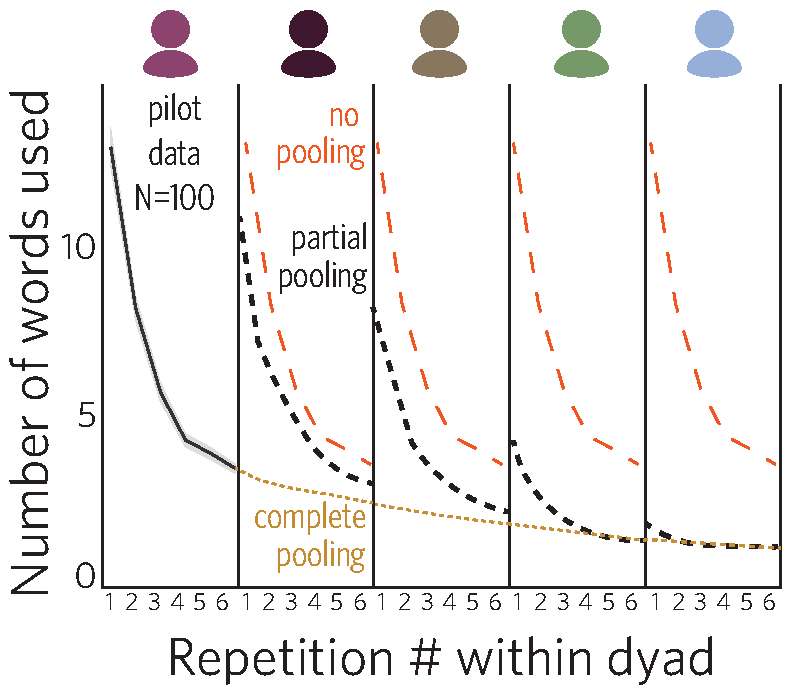
\includegraphics[scale=.5]{task1_predictions.pdf}
  \caption{Predictions}% tying individual cognition to population-level patterns}
  \label{fig:task1predictions}
\end{figure}
We will test these predictions using a mixed-effects regression of partner number on ``reversion size'' (the difference in number of words between the final descriptions on one repetition and the initial ones on the next), with maximum random-effect structure including item-effects at the object and speaker level.  
Only the partial pooling model predicts a significant decrease in reversion over successive partners. 
Preliminary support for this signature was reported by \shortciteA{fay_interactive_2010} in a Pictionary task where participants used sketches to communicate verbal concepts instead of using words to refer to visual targets, and the measure of interest was the  complexity of the drawings \cite<see also>{garrod_conversation_1994}.

\section{\bf Acknowledgments}
\small

\bibliography{ref}
\bibliographystyle{apacite}


\end{document}  
